\documentclass[../../main.tex]{subfiles}
\graphicspath{{../../image/}{../../figure/}}
\begin{document}

\section{超声速等熵气流绕凸角}\label{section:ch18-超声速绕凸角}

在 $x$-$y$ 平面的上半平面，考虑气体的等熵流动：上游状态为 $(\rho_f,u_f,0)$，$u_f>0$，撞击一个角顶在原点、斜率为 $\tan\omega$ 的固体凸壁（见图\cref{figure:ch18-绕凸角激波}）。等价地，可把这一构型看作气流绕过顶点角为 $2\omega$ 的固体楔的（关于 $x$ 轴对称的）上半部分。

我们考察以图\cref{figure:ch18-绕凸角激波}所示波型作定常流动的可行性，即以一道斜率 $s>\tan\omega$ 的 3-激波连接两个常状态 $(\rho_f,u_f,0)$ 与 $(\rho_b,u_b,v_b)$。为此，$(\rho_f,u_f,0)$ 需为超声速，而 $(u_b,v_b)$ 应落在 $(\rho_f,u_f,0)$ 的激波极曲线上，并须满足固体凸壁施加的边界条件，即 $v_b=u_b\tan\omega$，使法向速度分量在凸壁上为零。参照\cref{figure:ch18-激波极曲线}，确定角 $\omega_0$，使满足上述条件的波型数目为：当 $\omega>\omega_0$ 时为零，当 $\omega=\omega_0$ 时为一，当 $\omega<\omega_0$ 时为二。在后一情形，按惯例把强度较大的激波称为强激波，强度较小者称为弱激波。这不应与本书前面出现的“弱”字用法混淆；事实上，此处的弱激波本身可以相当强。

\begin{figure}[ht]
\centering
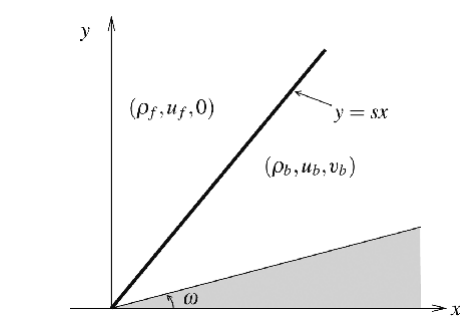
\includegraphics[width=0.85\textwidth]{ch18-fig04-01.png}
\caption{超声速气流绕斜率 $\tan\omega$ 的凸壁，由一道 3-激波连接上游状态 $(\rho_f,u_f,0)$ 与后状态 $(\rho_b,u_b,v_b)$。}
\label{figure:ch18-绕凸角激波}
\end{figure}

\begin{figure}[ht]
\centering
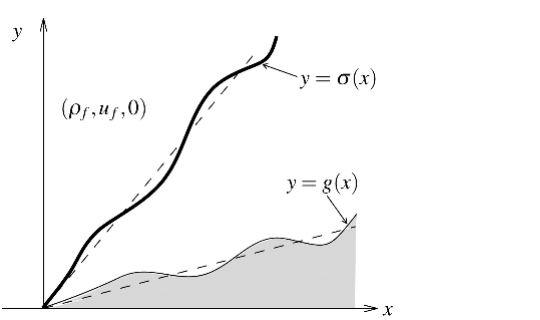
\includegraphics[width=0.85\textwidth]{ch18-fig04-02.png}
\caption{当凸壁形状由直线 $y=x\tan\omega$ 扰动为曲线 $y=g(x)$ 时，激波变为弯曲曲线 $y=\sigma(x)$。}
\label{figure:ch18-扰动凸壁}
\end{figure}

无旋流动情形下的情形完全相同（只是 $\omega_0$ 不同）。

强激波与弱激波中哪一个（或二者）物理可容，在过去六十年间争论激烈，但至今尚未以确定方式了结。基于实验与数值证据或稳定性考虑，有充分迹象表明物理可容的是弱激波解。当然，稳定性有不同的概念，甚至强激波解也满足某些稳定性准则。这些问题的详细讨论见\cref{section:ch18-注记}所引文献。此处我们只试图通过勾勒两条考察弱激波解稳定性的不同途径，略微品尝一下这场持续的讨论。

由\cref{section:ch18-定常平面等熵气流}中的推导可知，当 $\omega$ 不超过某个临界值 $\omega_{cr}\in(0,\omega_0)$ 时，弱激波解的后状态 $(\rho_b,u_b,v_b)$ 为超声速。我们此处研究的正是这一情形。

第一个检验是：超声速弱激波解在凸壁几何扰动下的稳定性。于是，把直凸壁 $y=x\tan\omega$，$x\geqslant0$，扰动为曲线 $y=g(x)$，$x\geqslant0$，其中 $g$ 是 $[0,\infty)$ 上的 $C^1$ 函数，满足 $g(0)=0$，$g'(0)=\tan\omega$，且 $g'$ 在 $[0,\infty)$ 上有界变差；见图\cref{figure:ch18-扰动凸壁}。我们的任务是确定一道定常等熵流动，给定超声速上游状态 $(\rho_f,u_f,0)$，$u_f>0$，撞击上述障碍。设 $\omega\in(0,\omega_{cr})$，使当 $g(x)=x\tan\omega$ 时，这一流动由图\cref{figure:ch18-绕凸角激波}所示的超声速弱激波解确定。

\begin{theorem}[弱激波解的结构稳定性]\label{theorem:ch18-弱激波稳定性}
存在正常数 $\varepsilon$ 与 $a$，使得当
\begin{align}
TV_{[0,\infty)}g'(\cdot)<\varepsilon
\label{align:ch18-1841}
\end{align}
时，存在凸壁上方的定常等熵流动 $(\rho,u,v)$，即定义在区域 $\{(x,y):0\leqslant x<\infty,\ g(x)\leqslant y<\infty\}$ 上，并具有如下结构：
\begin{enumerate}
\item\label{item:ch18-弱激波-a} 存在 $[0,\infty)$ 上的 Lipschitz 曲线 $y=\sigma(x)$，满足 $\sigma(0)=0$，$\sigma'(0+)=s$，它是一道超声速弱激波。$\sigma$ 的斜率 $\sigma'$ 是 $[0,\infty)$ 上的有界变差函数，且
\begin{align}
TV_{[0,\infty)}\sigma'(\cdot)\leqslant a\,TV_{[0,\infty)}g'(\cdot).
\label{align:ch18-1842}
\end{align}
\item\label{item:ch18-弱激波-b} 在区域 $\{(x,y):0\leqslant x<\infty,\ \sigma(x)<y<\infty\}$ 上，$(\rho,u,v)=(\rho_f,u_f,0)$。
\item\label{item:ch18-弱激波-c} 在区域 $\{(x,y):0<x<\infty,\ g(x)\leqslant y<\sigma(x)\}$ 上，$(\rho,u,v)$ 是\eqref{align:ch18-1821}的 $BV$ 解，其在曲线 $y=g(x)$ 上的迹满足边界条件
\begin{align}
v(x,g(x))=g'(x)u(x,g(x)),
\label{align:ch18-1843}
\end{align}
它表示法向于刚性障碍的速度分量为零。
\end{enumerate}
总变差很小，由 $g'$ 的总变差控制：
\begin{align}
TV_{[g(x),\infty)}(\rho(x,\cdot),u(x,\cdot),v(x,\cdot))\leqslant a\,TV_{[0,\infty)}g'(\cdot),
\label{align:ch18-1844}
\end{align}
对每个 $x\in(0,\infty)$ 成立。最后，
\begin{align}
\lim_{x\to\infty}\frac{v(x,y)}{u(x,y)}=\lim_{x\to\infty}g'(x),
\label{align:ch18-1845}
\end{align}
对 $y\in[g(x),\sigma(x)]$ 一致成立。
\end{theorem}

上述命题冗长而技术性的证明，载于\cref{section:ch18-注记}所引文献，是构造性的，采用了将随机选取法适用于本设定的一种变形。

我们的下一任务是给出证据：定常超声速弱激波解在动力学上是稳定的，即它描述了非定常流动在区域 $\{(x,y):0\leqslant x<\infty,\ x\tan\omega\leqslant y<\infty\}$ 上、具边界条件
\begin{align}
(\rho,u,v)(0,y,t)=(\rho_f,u_f,0),\qquad 0\leqslant y<\infty,\ 0<t<\infty,
\label{align:ch18-1846}
\end{align}
\begin{align}
v(x,x\tan\omega,t)=u(x,x\tan\omega,t)\tan\omega,\qquad 0<x<\infty,\ 0<t<\infty,
\label{align:ch18-1847}
\end{align}
与初始条件
\begin{align}
(\rho,u,v)(x,y,0)=(\rho_f,u_f,0),\qquad 0\leqslant x<\infty,\ x\tan\omega<y<\infty
\label{align:ch18-1848}
\end{align}
时的长时间行为。

我们将在绝热指数 $\gamma>1$、状态方程为\eqref{align:ch18-18317}的理想气体势流范围内，构造满足上述规格的流动。数据假设为：$(\rho_f,u_f,0)$，$u_f>0$，是超声速状态；且 $\omega<\omega_{cr}$，此时前面状态为 $(\rho_f,u_f,0)$ 的弱定常激波之后状态 $(\rho_b,u_b,v_b)$，$v_b/u_b=\tan\omega$，也为超声速。所期望的结果是：当 $t\to\infty$ 时，该非定常流动收敛到图\cref{figure:ch18-绕凸角激波}所示的定常流动。

由于区域的几何以及所给初边值数据在坐标伸缩下的不变性，所期望的流动是自相似的，如\cref{section:ch18-自相似无旋等熵气流}中讨论的那样，即 $\rho,u,v$ 与伪势 $\chi$ 是两个变量 $\xi=x/t$、$\zeta=y/t$ 的函数。特别地，如\cref{section:ch18-自相似无旋等熵气流}所说明，连接状态 $(\rho_f,u_f,0)$ 与 $(\rho_b,u_b,v_b)$ 的定常超声速激波，在 $\xi$-$\zeta$ 平面中表现为一条过原点的直线。

在远离原点的点，拐角效应不会立刻感受到，因而短期内初始与边界条件在凸壁上的相互作用将产生一道反射超声速激波，斜率为 $\tan\omega$，连接前面状态 $(\rho_f,u_f,0)$ 与某状态 $(\rho_d,u_d,v_d)$。该激波的方程形式为
\begin{align}
\zeta=(\xi+\ell)\tan\omega,
\label{align:ch18-1849}
\end{align}
其中 $\ell>0$ 为待下方确定的常数。由边界条件\eqref{align:ch18-1847}，向量 $(u_d,v_d)$ 必与激波相切，$v_d/u_d=\tan\omega$。此外，由于速度切向分量跨过激波连续，该向量必与 $(u_f,0)$ 的切向分量重合。故
\begin{align}
u_d=u_f\cos^2\omega,\qquad v_d=u_f\sin\omega\cos\omega,\qquad
\sqrt{u_d^2+v_d^2}=u_f\cos\omega.
\label{align:ch18-18410}
\end{align}
为确定剩余参数 $\rho_d$ 与 $\ell$，借助表达质量守恒的 Rankine--Hugoniot 条件\eqref{align:ch18-18315}，它在此退化为
\begin{align}
\ell(\rho_d-\rho_f)=\rho_fu_f,
\label{align:ch18-18411}
\end{align}
以及由 Bernoulli 方程决定的\eqref{align:ch18-18316}，它给出
\begin{align}
\ell u_f\sin^2\omega=\rho_d^{\gamma-1}-\rho_f^{\gamma-1}-\frac12 u_f^2\sin^2\omega.
\label{align:ch18-18412}
\end{align}
联立\eqref{align:ch18-18411}与\eqref{align:ch18-18412}，得方程
\begin{align}
\frac{\bigl(\rho_d^{\gamma-1}-\rho_f^{\gamma-1}\bigr)(\rho_d-\rho_f)}{\rho_d+\rho_f}
=\frac12 u_f^2\sin^2\omega,
\label{align:ch18-18413}
\end{align}
它有唯一解 $\rho_d$ 满足可容性条件 $\rho_d>\rho_f$。最后由\eqref{align:ch18-18411}定出 $\ell$。

声速圆的概念已在\cref{section:ch18-自相似无旋等熵气流}中引入。状态 $(\rho_b,u_b,v_b)$ 的声速圆以位于凸壁上的点 $(u_b,v_b)$ 为圆心，半径为 $\sqrt{\gamma-1}\,\rho_b^{\frac{\gamma-1}{2}}$。由于 $(\rho_b,u_b,v_b)$ 超声速，原点 $\xi=\zeta=0$ 位于该圆之外，但定常激波 $\zeta=s\xi$ 与圆交于两点，其中离原点最近者记为 $(\xi_L,\zeta_L)$。类似地，状态 $(\rho_d,u_d,v_d)$ 的声速圆以位于凸壁上的点 $(u_d,v_d)$ 为圆心，半径为 $\sqrt{\gamma-1}\,\rho_d^{\frac{\gamma-1}{2}}$，它与激波 $\zeta=(\xi+\ell)\tan\omega$ 交于两点，其中离原点较远者记为 $(\xi_R,\zeta_R)$。

\begin{figure}[ht]
\centering
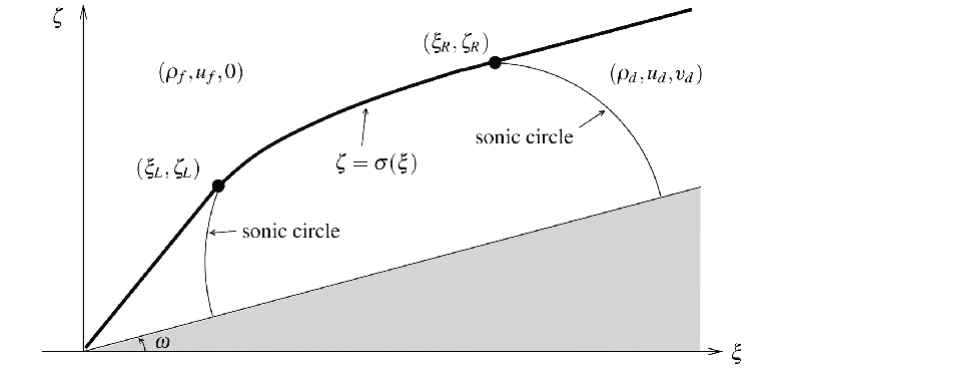
\includegraphics[width=0.9\textwidth]{ch18-fig04-03.png}
\caption{跨声速激波 $\zeta=\sigma(\xi)$：从定常超声速段 $\sigma(\xi)=s\xi$ 过渡到运动超声速段 $\sigma(\xi)=(\xi+\ell)\tan\omega$，中间跨声速段夹在两个声速圆之间。}
\label{figure:ch18-Prandtl自相似流}
\end{figure}

\begin{theorem}[Prandtl 问题的解]\label{theorem:ch18-Prandtl问题}
在上述假设下，存在一分段光滑、自相似的流动 $(\rho,u,v)$，其构型如图\cref{figure:ch18-Prandtl自相似流}所示，并具有如下结构：
\begin{enumerate}
\item\label{item:ch18-Prandtl-a} 它含单一激波 $\zeta=\sigma(\xi)$，其中 $\sigma\in C^1[0,\infty)$。当 $0<\xi<\xi_L$ 时，激波是定常超声速的，$\sigma(\xi)=s\xi$，连接 $(\rho_f,u_f,0)$ 与 $(\rho_b,u_b,v_b)$；当 $\xi_L<\xi<\xi_R$ 时，激波跨声速；当 $\xi_R<\xi<\infty$ 时，激波超声速，$\sigma(\xi)=(\xi+\ell)\tan\omega$，以速率 $\ell\sin\omega$ 运动，连接 $(\rho_f,u_f,0)$ 与 $(\rho_d,u_d,v_d)$。在 $(\xi_L,\xi_R)$ 上，$\sigma$ 为 $C^3$ 且凸。
\item\label{item:ch18-Prandtl-b} 激波前方的区域是常状态 $(\rho_f,u_f,0)$。
\item\label{item:ch18-Prandtl-c} 激波定常超声速部分后方、位于 $(\rho_b,u_b,v_b)$ 的声速圆之外的区域，是常状态 $(\rho_b,u_b,v_b)$。
\item\label{item:ch18-Prandtl-d} 激波运动超声速部分后方、位于 $(\rho_d,u_d,v_d)$ 的声速圆之外的区域，是常状态 $(\rho_d,u_d,v_d)$。
\item\label{item:ch18-Prandtl-e} 在激波跨声速部分后方、左以 $(\rho_b,u_b,v_b)$ 的声速圆为界、右以 $(\rho_d,u_d,v_d)$ 的声速圆为界的区域内，$(\rho,u,v)$ 是光滑函数，$(u,v)$ 由光滑伪势 $\chi$ 导出：
\begin{align}
u=\chi_\xi+\xi,\qquad v=\chi_\zeta+\zeta,
\label{align:ch18-18414}
\end{align}
并满足偏微分方程
\begin{align}
\nabla\cdot\left[\left(\rho_0^{\gamma-1}-\chi-\frac12|\nabla\chi|^2\right)^{\frac{1}{\gamma-1}}\nabla\chi\right]
+2\left(\rho_0^{\gamma-1}-\chi-\frac12|\nabla\chi|^2\right)^{\frac{1}{\gamma-1}}=0,
\label{align:ch18-18415}
\end{align}
它是椭圆型的。
\end{enumerate}
\end{theorem}

双曲区域中密度与速度场的构造已在上面阐述。然后借助\eqref{align:ch18-1839}容易确定伪势 $\chi$。常数的选取应使 $\chi$ 跨过激波连续。特别地，在激波前方区域，
\begin{align}
\chi=u_f\xi-\frac12(\xi^2+\zeta^2).
\label{align:ch18-18416}
\end{align}
然后在激波定常部分后方、位于 $(\rho_b,u_b,v_b)$ 的声速圆之外的区域，
\begin{align}
\chi=u_b\xi+v_b\zeta-\frac12(\xi^2+\zeta^2).
\label{align:ch18-18417}
\end{align}
最后，在激波运动超声速部分后方、位于 $(\rho_d,u_d,v_d)$ 的声速圆之外的区域，由\eqref{align:ch18-1849}与\eqref{align:ch18-18410}得
\begin{align}
\chi=u_d\xi+v_d\zeta-\frac12(\xi^2+\zeta^2)-\frac12\ell u_f\sin 2\omega.
\label{align:ch18-18418}
\end{align}
剩下要做的是在椭圆区域中构造 $\chi$，即方程\eqref{align:ch18-18415}在如下边界条件下的解。沿凸壁，$\partial\chi/\partial\nu=0$，使速度的法向分量为零。沿两个声速圆的弧段，$\chi$ 及其一阶导数由速度场跨过这些曲线连续的要求给定。最后，跳跃条件\eqref{align:ch18-18315}与\eqref{align:ch18-18316}必须跨过激波成立。求解这一问题并非易事。首先，激波跨声速部分在区间 $(\xi_L,\xi_R)$ 上的图像事先未知，它是一个须作为解的一部分来确定的自由边界。另一主要困难是：椭圆性沿声速圆弧退化，而同时在那里又给定了 Dirichlet 与 Neuman 边界数据。为克服这些障碍所需的艰苦而技术性的分析超出了本书范围。\cref{theorem:ch18-Prandtl问题}的证明见\cref{section:ch18-注记}所引文献。

当 $\omega$ 增大时，与原点相邻的超声速区域缩小，并在 $\omega=\omega_{cr}$ 时消失，此时跨声速激波从凸壁根部发出。即使 $\omega$ 继续增大超过 $\omega_{cr}$，只要在 $[\omega_{cr},\omega_0)$ 范围内，这一构型仍持续。见\cref{section:ch18-注记}所引文献。

显然，图\cref{figure:ch18-Prandtl自相似流}所示的自相似流动，转换回原始变量 $(x,y,t)$ 后，当 $t\to\infty$ 趋于图\cref{figure:ch18-绕凸角激波}所示的定常流动。

\end{document}
